\newcommand{\footnoteSS}[1]{\footnote{
\renewcommand{\baselinestretch}{1.0} \footnotesize \setlength{\oddsidemargin}{-0.4in}
\setlength{\evensidemargin}{-0.4in} \setlength{\textwidth}{7.2in}
#1}}


\documentclass[12pt,fleqn]{article}
%%%%%%%%%%%%%%%%%%%%%%%%%%%%%%%%%%%%%%%%%%%%%%%%%%%%%%%%%%%%%%%%%%%%%%%%%%%%%%%%%%%%%%%%%%%%%%%%%%%%%%%%%%%%%%%%%%%%%%%%%%%%%%%%%%%%%%%%%%%%%%%%%%%%%%%%%%%%%%%%%%%%%%%%%%%%%%%%%%%%%%%%%%%%%%%%%%%%%%%%%%%%%%%%%%%%%%%%%%%%%%%%%%%%%%%%%%%%%%%%%%%%%%%%%%%%
\usepackage{amsmath}
\usepackage{slashed}
\usepackage{amssymb}
\usepackage{graphicx}
\usepackage{chicago}

\setcounter{MaxMatrixCols}{10}
%TCIDATA{OutputFilter=Latex.dll}
%TCIDATA{Version=5.50.0.2960}
%TCIDATA{<META NAME="SaveForMode" CONTENT="1">}
%TCIDATA{BibliographyScheme=BibTeX}
%TCIDATA{LastRevised=Friday, October 07, 2011 15:01:21}
%TCIDATA{<META NAME="GraphicsSave" CONTENT="32">}

\setlength{\paperwidth}{8.5in} \setlength{\paperheight}{11.0in}
\setlength{\topmargin}{0.0in} \setlength{\headheight}{0.4in}
\setlength{\headsep}{0.0in} \setlength{\textwidth}{7.2in}
\setlength{\textheight}{8.5in} \setlength{\oddsidemargin}{0.0in}
\setlength{\oddsidemargin}{-0.4in}
\setlength{\evensidemargin}{-0.4in}
\renewcommand{\baselinestretch}{1.5}
\renewcommand{\textfraction}{0.33}

\input{tcilatex}

\begin{document}



\section{\protect\normalsize A Monte Carlo exercise: the correlation between
consumption and investment}

{\normalsize As illustrated above, in a one-sector model a permanent
increase in the level of the IST shock, $Z_{s},$ would initially boost
investment and aggregate output while compressing consumption. Conversely,
in a two-sector model with our alternative calibration, the corresponding
increase in the MFP shock specific to the machinery sector, $A_{s},$ would
imply positive conditional comovement between consumption and investment as
well as between consumption and aggregate output. }

{\normalsize \citeN{fisher2006} disentangles the effects of sector-specific
and economy-wide MFP shocks. In the identification scheme of %
\citeN{fisher2006}, as in that of \citeN{gali1999}, it is assumed that
permanent economy-wide technology shocks are the only shocks to influence
the level of labor productivity in the long run and that sectoral technology
shocks are the only ones to affect the relative price of machinery in the
long run. \citeN{fisher2006} wrote down a one-sector model with economy-wide
MFP shocks and IST shocks to motivate such a scheme. However, he also noted
that under some assumptions, including that of equal factor shares across
sectors, the scheme would also be consistent with a two sector model
producing consumption and investment. Like us, \citeN{basu2010}, stress that
factor shares vary substantially across sectors. They conclude that the
identification scheme in \citeN{fisher2006} is inconsistent with such
differences. }

{\normalsize To investigate this issue, we vary the technology in the
machinery and non-machinery sectors to reflect the effects of an
economy-wide MFP shock $\tilde{G}_s$:
\begin{eqnarray}
&& Y^A_{Ms}= \left( \tilde{G}_s \tilde{A}_s L_{Ms}\right)
^{1-\alpha_{M}^{E}-\alpha _{M}^{S}}\left( K_{Ms}^{E}\right) ^{\alpha
_{M}^{E}}\left( K_{Ms}^{S}\right) ^{\alpha_{M}^{S}}, \\
&& Y^A_{Ns}= \left( \tilde{G}_s L_{Ns}\right) ^{1-\alpha_{N}^{E}-\alpha
_{M}^{S}}\left( K_{Ns}^{E}\right) ^{\alpha _{N}^{E}}\left( K_{Ns}^{S}\right)
^{\alpha_{N}^{S}}.
\end{eqnarray}
The term $\tilde{A}_s$ represents MFP shocks that are specific to the
machinery sector. Notice that $\tilde{G}_s$ and $\tilde{A}_s$ are
labor-augmenting and that $\tilde{A}_s^{1-\alpha_{M}^{E}-\alpha _{M}^{S}}$
assumes the role played by $A_s$ in Section 2.1. }

{\normalsize We find that in fact the scheme devised by \citeN{fisher2006}
is consistent with a less restrictive set of assumptions than his. As Figure~%
\ref{figure_test} reveals, under the calibration with all the departures
from aggregate equivalence, including substantially different factor shares
across sectors, economy-wide MFP shocks do not affect relative prices in the
long run.\footnoteSS{%
Section~\ref{appendixb} of the appendix derives the same result analytically
for a special case of our model with complete specialization in the assembly
of final goods.} }

{\normalsize Having established that the key identifying restrictions in %
\citeN{fisher2006} do not contradict the assumptions in our two-sector
model, we proceed to use his methodology to investigate the co-movement
between consumption and investment conditional on shocks that move the
relative price of investment permanently. The only variables included in the
VAR estimated in \citeN{fisher2006} are the growth rate of the relative
price of investment, the growth rate of per capita labor productivity and
the level of hours worked per capita. To study the correlation between
private consumption and equipment investment we append these two variables
in per capita terms to the VAR we re-estimate. }

{\normalsize Several recent papers have modified the empirical strategy in %
\citeN{fisher2006} to replace labor productivity growth in the VAR with the
growth of TFP measures obtained from aggregate growth accounting exercises.
See, for instance, \citeN{beaudry2009}, \citeN{schmitt2011}, and %
\citeN{sims2011}. We continue to use labor productivity growth since the
conditions for aggregation underlying those TFP measures do not hold in our
model. }

{\normalsize The estimation sample runs from 1983Q3 to 2008Q3 to avoid
possible breaks in the data associated with dramatic changes in monetary
policy, such as the Volker disinflation at one end and the zero lower bound
on the Federal Funds rate at the other.\footnoteSS{%
The relative price of investment is constructed as the ratio between the
implicit deflator for equipment investment from Tables 1.1.5 (Gross Domestic
Product) and Tables 1.1.3 (Real Gross Domestic Product) of the National
Income and Product Accounts and the deflator for non-equipment an software
(the remainder of U.S. GDP). We construct the latter deflator netting
equipment and software prices from the deflator for overall GDP using
Laspeyeres's formula. Whenever we express variables in per capita terms, we
use data from the Current Population Survey on the Civilian,
non-Institutional population aged 16 and over. The labor productivity series
and the series on hours worked come from the Productivity Release of the
Bureau of Labor Statistics and relate to the non-farm business sector. The
series for private consumption and for equipment investment come from the
National Income and Products Accounts.} Like \citeN{fisher2006}, we are only
identifying the shocks to the first two variables. }

{\normalsize The solid lines in Figure \ref{figure_datavar} show the effects
on output, consumption, and investment of a one-standard deviation shock
estimated in the VAR to reduce the price of investment permanently. The
point estimate for the decline in the relative price (not shown) is 2
percent. The dotted lines show 90\% bootstrap confidence intervals. While
the confidence intervals are strikingly large, they exclude a negative
response of consumption. From the impulse responses it is clear that there
is conditional comovement between both consumption and investment as well as
consumption and aggregate production. The point estimate for the population
correlation between consumption and investment at business cycle frequencies
is 0.98. The analogous statistic for consumption and production is 0.97.%
\footnoteSS{%
We used a bandpass filter to isolate the oscillations with frequencies
between 6 and 32 quarters, typically used to define the business cycle.} }

\subsection{\protect\normalsize A Monte Carlo experiment}

{\normalsize To verify that we can effectively discriminate between the
one-sector model with IST shocks and our two-sector model based on the the
empirical evidence just presented, we use a Monte Carlo experiment. We apply
the same identification scheme to a VAR estimated on data generated from
both models to obtain the sampling distribution of the correlation between
consumption and aggregate production conditional on shocks that move the
relative price of investment permanently. }

{\normalsize For the Monte Carlo experiment, we need to expand the menu of
shocks considered beyond neutral and sectoral technology shocks in order to
avoid a statistical singularity. Accordingly, we modify the utility function
of households in Equation (\ref{utility}) as follows:
\begin{equation}
\sum_{s=t}^{\infty }\beta ^{s-t} \left[ \frac{\left( C_{s} -F_{cs}\right)
^{1-\gamma_c }-1}{1-\gamma_c } - \gamma_{0} \frac{\left( L_{s}
-F_{ls}\right) ^{1-\gamma_l }-1}{1-\gamma_l } \right],  \label{utility2}
\end{equation}
Under this alternative, utility also depends on the aggregate labor supply $%
L_s$. In addition, $F_{cs}$ and $F_{ls}$ represent, respectively, a
stationary consumption preference shock and a stationary labor supply shock.
The market clearing conditions for the the labor market now implies that
sectoral labor demand needs to sum to the aggregate labor supply $L_s$.
Because the focus of the exercise is on the correlation between consumption
and output, we can eliminate the investment growth series from the VAR in
the Monte Carlo exercise.\footnoteSS{%
We verified that the VAR results from the observed U.S. data would be little
changed upon excluding the series for equipment investment.} }

{\normalsize To run the Monte Carlo experiment, we need to take a stand on
the relative importance of the various sources of fluctuations and on the
additional parameters in the utility function. These choices are summarized
in Table \ref{additional_calibration}.\footnoteSS{%
As in the previous sections of the paper, all other parameters are reported
in Table \ref{table_constantparameters} for the one-sector model and in
Table \ref{table_changed_parameters} for our two-sector model.} We continue
to consider unit root shocks to the level of sectoral and neutral
technology. We size the standard deviation of sectoral technology shocks
(either IST shocks in the one-sector model or sectoral MFP shocks in the
two-sector model) to match the 2 percent long-run decline for the relative
price of investment estimated in the VAR. Similarly, the standard deviation
of neutral technology shocks is chosen to match the long-run increase in
aggregate labor productivity equal to 0.34. The AR(1) coefficients and the
standard deviations for the shock processes governing the consumption
preference shock and the labor supply shock, as well the parameter $\gamma_l$
are chosen using the simulated method of moments. The distance function we
use assigns equal weights to the share of the population variance explained
by technology shocks (the sum of the contribution from sectoral and neutral
shocks) for each of the five variables included in the data VAR (growth of
the relative price of investment, labor productivity growth, level of hours
worked, growth of consumption, and growth of investment). We choose
parameters to minimize the distance between the point estimates from the VAR
and the model implied values for the same moments.\footnoteSS{%
The one-sector model implies that all variation of the relative price of
investment explained by technology shocks. This amounts having one fewer
moment condition. Accordingly, we reduce the number of parameters by setting
$\gamma_l$ at the same value as for the two-sector model.} Finally, we set $%
\gamma_{0}$ to normalize aggregate hours worked to 1 in the non-stochastic
steady state, the same value for aggregate hours worked used in the
simulations presented in previous sections. }

{\normalsize Using each model in turn, we generate 1000 samples of length
equal to that of the observed sample. For each sample we re-estimate a VAR.
Figure~\ref{figure_samplingdistribution} presents the sampling distribution
of the correlation between consumption and aggregate production at business
cycle frequencies conditional on shocks that move permanently the price of
investment. The sampling distributions for both models are wide,
underscoring that the VAR with long-run restrictions only yields imprecise
estimates in small samples. However, the distribution from the two-sector
model is skewed to the right of the range. Accordingly, the two-sector model
is a better candidate to generate a correlation equal to 0.97 estimated on
observed U.S. data. Conditioning on shocks that affect the price of
investment in the long run, the probability of observing a correlation
between consumption and production at business cycle frequencies exceeding
0.9 is 0.35 when the two sector model is the data-generating process and
only 0.01 for the one-sector model. We interpret this finding as evidence
that our two-sector model is a better candidate for reconciling the strong
conditional comovement uncovered by the VAR estimates based on observed U.S.
data. }

\section{Appendix: The Long-Run Response of Relative Prices and Labor
Productivity to Technology Shocks (not intended for publication)}
\label{appendixb}

We derive steady-state relationships for a special case of the model
in the main body of the paper. Specifically, the model includes only
one stock of capital in each sector; both capital and labor are
perfectly mobile; there is complete specialization in the assembly
of consumption and investment. Some important implications of the
model for the identification of technology shocks through relative
prices carry through to the richer model in the paper, as supported
by numerical simulations presented there. Namely, relative prices
respond only to sector-specific shocks while labor productivity
(aggregated at constant prices or in units of consumption) responds
to both equiproportionate sectoral shocks as well as to
sector-specific shocks. Hence, our two sector model is consistent
with the identification scheme in \citeN{fisher2006} despite
different factor input shares across sectors.

\subsection{The model}

In period $t$, the representative household supplies a fixed amount
of labor
$L$, and maximizes the intertemporal utility function%
\begin{equation}
\max_{C_{t},I_{t},K_{Nt},K_{Mt},B_{t}}\sum_{s=t}^{\infty }\beta
^{s-t}\log C_{s},
\end{equation}%
subject to the budget constraint
\begin{equation}
W_{s}L+R_{Ms}K_{Ms}+R_{Ns}K_{Ns}+\rho
_{s-1}B_{s-1}=P_{Ns}C_{s}+P_{Mt}I_{t}+B_{t},
\end{equation}%
and subject to the following law of motion for the accumulation of
capital
\begin{equation}
K_{Ms+1}+K_{Ns+1}=(1-\delta )(K_{Ms}+K_{Ns})+I_{s}.
\end{equation}

There is complete specialization in the assembly of consumption and
investment goods. Hence, $I_{t}=Y_{Mt}$, and $C_{t}=Y_{Nt}$. In each
sector, perfectly competitive firms minimize production costs to
meet demand subject to the technology constraint as reflected in the
following Lagrangian
problems:%
\begin{equation}
\min_{K_{Mt},L_{Mt},P_{Mt}}R_{Mt}K_{Mt}+W_{t}L_{Mt}+P_{Mt}(Y_{Mt}-K_{Mt}^{%
\alpha _{M}}\left( A_{t}G_t L_{Mt}\right) ^{1-\alpha _{M}}),
\end{equation}%
\begin{equation}
\min_{K_{Nt},L_{Nt},P_{Nt}}R_{Nt}K_{Nt}+W_{t}L_{Nt}+P_{Nt}(Y_{Nt}-K_{Nt}^{%
\alpha _{N}}\left( G_{t}L_{Nt}\right) ^{1-\alpha _{N}}).
\end{equation}%
In addition to satisfying the first-order conditions given above for
the optimization problems of households and firms, an equilibrium in
the model is such that all factor markets and product markets clear.

\begin{table}[tbp]
\caption{Steady State Restrictions} \label{SSrestrictions}\center
\begin{tabular}{|l|c|l|c|}
\hline
I) & $\frac{R_{N}}{P_{N}C}-\frac{P_{M}}{P_{N}C}+\beta \frac{P_{M}}{P_{N}C}%
(1-\delta)=0$ & II) & $R_{Nt}=R_{Mt}$ \\
III) & $R_{M}=P_{M}\alpha _{M}\frac{Y_{M}}{K_{M}}$ & IV) &
$W=P_{M}(1-\alpha
_{M})\frac{Y_{M}}{L_{M}}$ \\
V) & $R_{N}=P_{N}\alpha _{N}\frac{Y_{N}}{K_{N}}$ & VI) &
$W=P_{N}(1-\alpha
_{N})\frac{Y_{N}}{L_{N}}$ \\
VII) & $Y_{M}=K_{M}^{\alpha _{M}}(A G L_{M})^{1-\alpha _{M}}$ & VIII) & $%
Y_{N}=K_{N}^{\alpha _{N}}(G L_{N})^{1-\alpha _{N}}$ \\
IX) & $Y_{M}=I$ & X) & $Y_{N}=C$ \\
XI) & $L_{M}+L_{N}=L$ & XII) & $K_M+K_N = \frac{1}{\delta} Y_M$ \\
\hline
\end{tabular}%
\end{table}

\subsection{The Long-Run Response of Relative Prices}

From I) and II) in Table \ref{SSrestrictions}
\begin{equation}
R_{M}=R_{N}=P_{M}\left( 1-\beta (1-\delta )\right) .  \label{SSR}
\end{equation}%
From III) and VII), and from V) and VIII) in Table
\ref{SSrestrictions}, we obtain, respectively, that:
\begin{equation}
\frac{Y_{M}}{L_{M}}=AG\left( \alpha _{M}\frac{P_{M}}{R_{M}}\right) ^{%
\frac{\alpha _{M}}{1-\alpha _{M}}},  \label{SSYm}
\end{equation}%
\begin{equation}
\frac{Y_{N}}{L_{N}}=G\left( \alpha _{N}\frac{P_{N}}{R_{N}}\right) ^{%
\frac{\alpha _{N}}{1-\alpha _{N}}}.  \label{SSYn}
\end{equation}%
Next, consider IV) and VI) in Table \ref{SSrestrictions}:
\begin{equation}
\frac{P_{M}}{P_{N}}=\frac{(1-\alpha _{N})}{(1-\alpha _{M})}\frac{Y_{N}}{L_{N}%
}\frac{L_{M}}{Y_{M}}.  \label{SSPmPn}
\end{equation}%
Substituting equations \ref{SSR}, \ref{SSYm}, and \ref{SSYn} into equation %
\ref{SSPmPn}, one can solve for $\frac{P_{M}}{P_{N}}$ in terms of
parameters and the level of sector-specific technology $A$:
\begin{equation}
\frac{P_{M}}{P_{N}}=\psi _{1}\left( \frac{1}{A}\right) ^{1-\alpha
_{N}},\text{ \ where }\psi _{1}=\left( \frac{(1-\alpha _{N})}{(1-\alpha _{M})%
}\frac{\left( \alpha _{N}\frac{1}{\left( 1-\beta (1-\delta )\right)
}\right) ^{\frac{\alpha _{N}}{1-\alpha _{N}}}}{\left( \alpha
_{M}\frac{1}{\left(
1-\beta (1-\delta )\right) }\right) ^{\frac{\alpha _{M}}{1-\alpha _{M}}}}%
\right) ^{1-\alpha _{N}}.  \label{SSRelprice}
\end{equation}%
Thus, equiproportionate changes in technology in the two production sectors $%
M$ and $N$ will not affect relative prices. Variation in relative
prices at the sectoral level is a precondition for variation in
relative prices at the level of final goods. Thus, the result
derived here extends to the model in the main body of the paper with
incomplete sectoral specialization in the assembly of consumption
and investment goods, as reflected in the numerical simulations.

\subsection{The Long-Run Response of Labor Productivity}

Define labor productivity as:
\begin{equation}
\frac{Y_{Mt}+Y_{Nt}}{L}=\frac{Y_{Mt}}{L_{Mt}}\frac{L_{Mt}}{L}+\frac{Y_{Nt}}{%
L_{Nt}}\frac{L_{Nt}}{L}.
\end{equation}%
First work on obtaining $\frac{L_{Mt}}{L}$ and $\frac{L_{Nt}}{L}$.
Using V, VIII, \ref{SSR} and III, VII, \ref{SSR} one can obtain,
respectively:
\begin{equation}
\frac{K_{M}}{Y_{M}}=\frac{\alpha _{M}}{\left( 1-\beta (1-\delta
)\right) }, \label{SSKmYm}
\end{equation}%
\begin{equation}
\frac{K_{N}}{Y_{N}}=\frac{\alpha _{N}}{\left( 1-\beta (1-\delta )\right) }%
\frac{P_{N}}{P_{M}}.  \label{SSKnYn}
\end{equation}%
$\frac{K_{N}}{Y_{N}}$ can be related to technology levels through \ref%
{SSRelprice}. From XII, one has that:
\begin{equation}
\frac{K_{N}}{Y_{N}}\frac{Y_{N}}{Y_{M}}+\frac{K_{M}}{Y_{M}}=\frac{1}{\delta
},
\end{equation}%
which can be used with to \ref{SSKmYm} and \ref{SSKnYn} to solve for $\frac{%
Y_{N}}{Y_{M}}$:
\begin{equation}
\frac{Y_{N}}{Y_{M}}=\psi _{2}\frac{1}{A^{1-\alpha _{N}}},\text{ \
where \ }\psi _{2}=\psi _{1}\left( \frac{\left( 1-\beta
(1-\delta )\right) }{\delta \alpha _{N}}-\frac{\alpha _{M}}{\alpha _{N}}%
\right)
\end{equation}%
Combining IV, VI, and XI, one obtains:
\begin{equation}
\frac{L_{M}}{L}=\frac{(1-\alpha _{M})P_{Mt}Y_{Mt}}{(1-\alpha
_{N})P_{Nt}Y_{Nt}+(1-\alpha _{M})P_{Mt}Y_{Mt}},
\end{equation}%
which can be expressed as a function of parameters and technology
levels as:
\begin{equation}
\frac{L_{M}}{L}=\frac{(1-\alpha _{M})\psi _{1}}{(1-\alpha _{M})\psi
_{1}+(1-\alpha _{N})\psi _{2}},
\end{equation}%
and since $L_{N}+L_{M}=L$ once can see that:
\begin{equation}
\frac{L_{N}}{L}=\frac{(1-\alpha _{N})\psi _{2}}{(1-\alpha _{M})\psi
_{1}+(1-\alpha _{N})\psi _{2}}.
\end{equation}%
Next work on $\frac{Y_{Mt}}{L_{Mt}}$ and on $\frac{Y_{Nt}}{L_{Nt}}$.
Combining equations \ref{SSYm} and \ref{SSYn} with equation
\ref{SSR} yields:
\begin{equation}
\frac{Y_{M}}{L_{M}}=AG\left( \frac{\alpha _{M}}{\left( 1-\beta
(1-\delta )\right) }\right) ^{\frac{\alpha _{M}}{1-\alpha _{M}}},
\end{equation}%
\begin{equation}
\frac{Y_{N}}{L_{N}}=G\left( \frac{\alpha _{N}}{\left( 1-\beta
(1-\delta )\right) }\frac{P_{N}}{P_{M}}\right) ^{\frac{\alpha
_{N}}{1-\alpha _{N}}}.
\end{equation}%
Summing up, remembering that $\frac{P_{M}}{P_{N}}=\psi _{1}\left(
\frac{1}{A}\right) ^{1-\alpha _{N}}$ , one can see that at constant
prices:
\begin{eqnarray}
\frac{Y_{M}+Y_{N}}{L} &=&\frac{Y_{M}}{L_{M}}\frac{L_{M}}{L}+\frac{Y_{N}}{%
L_{N}}\frac{L_{N}}{L}= \nonumber \\ \label{SSlabprod} &&AG\left(
\frac{\alpha _{M}}{\left( 1-\beta (1-\delta )\right) }\right)
^{\frac{\alpha _{M}}{1-\alpha _{M}}}\frac{(1-\alpha _{M})\psi _{1}}{%
(1-\alpha _{M})\psi _{1}+(1-\alpha _{N})\psi _{2}} \\
&&+ A^{\alpha _{N}} G \left( \frac{\alpha _{N}}{\psi _{1}\left(
1-\beta (1-\delta )\right) }\right) ^{\frac{\alpha _{N}}{1-\alpha
_{N}}}\frac{(1-\alpha _{N})\psi _{2}}{(1-\alpha _{M})\psi
_{1}+(1-\alpha _{N})\psi _{2}}.
\end{eqnarray}%
Notice that Fisher defined aggregate labor productivity in terms of
consumption units
( i.e., $\frac{Y_{Mt}}{L_{Mt}}\frac{L_{Mt}}{L}\frac{P_{M}}{P_{N}}+\frac{Y_{N}%
}{L_{N}}\frac{L_{N}}{L}$) rather than at constant prices. Even under
that alternative aggregation, labor productivity remains a
log-linear function of both shocks. Based on equations
\ref{SSRelprice} and \ref{SSlabprod}, our model is consistent with
the scheme in \citeN{fisher2006}. 



\clearpage
\bibliographystyle{chicago}
\bibliography{bibliosearch}
\clearpage


\begin{figure}[tbp] \caption{Cumulative effects of all departures
from aggregate equivalence} \center \label{figure_test}
\includegraphics[scale=0.9]{figure_test.ps}
\end{figure}

\begin{figure}[tbp] \caption{The Effects of a Shock that Lowers the Price of Equipment
Investment Permanently --  Estimates from a VAR} \center
\label{figure_datavar}
\includegraphics[scale=0.8]{figure_datavar.ps}

\renewcommand{\baselinestretch}{1}
 \footnotesize \flushleft The solid lines show the point estimates for the
responses to a one standard deviation shock that lowers the relative
price of equipment investment permanently. The dotted lines show
90\% bootstrap confidence intervals.
\end{figure}


\begin{figure}[tbp] \center
\caption{Monte Carlo Results -- Sampling Distributions for the
Correlation Between Consumption and Aggregate Production at Business
Cycle Frequencies}  \label{figure_samplingdistribution}
\includegraphics[scale=0.9]{figure_samplingdistribution.ps}
\end{figure}


\end{document}